\documentclass[fleqn,8pt,t]{beamer}

\usepackage[english]{babel}
\usepackage[utf8]{inputenc}
\usepackage[T1]{fontenc}
%\usepackage{french} % Sommaire en début de document
%\usepackage[top=2cm, bottom=2cm, left=2cm, right=2cm]{geometry} % Marges

\usepackage{amsmath} % Maths
\usepackage{amsfonts} % Maths
\usepackage{amssymb} % Maths
\usepackage{stmaryrd} % Maths (crochets doubles)

%\usepackage{listings} % Mise en forme du code (pour Hoare) ## À REVOIR ###
%\usepackage{ifthen} % Structures If Then Else
\usepackage{theorem} % Styles supplémentaires pour théorèmes
\usepackage{url}
\usepackage{array}  % Tableaux évolués
\usepackage{multirow}  % Pour des colonnes sur plusieurs lignes

%\usepackage{enumerate} % Changer les puces des listes d'énumération
%\usepackage{setspace} % Changer les interlignes

%\usepackage{subfig} % Créer des sous-figures
%\usepackage{graphicx} % Importer des images

\usepackage{ulem}  % Pour l'attribut barré

\usepackage{comment}

% Police
\usepackage{lmodern}
%\usepackage{libertine}


\usepackage{tikz}

% Macros relatives à la traduction de PH avec arcs neutralisants vers PH à k-priorités fixes

% Macros générales
%\newcommand{\ie}{\textit{i.e.} }
\newcommand{\segm}[2]{\llbracket #1; #2 \rrbracket}
%\newcommand{\f}[1]{\mathsf{#1}}

% Notations générales pour PH
\newcommand{\PH}{\mathcal{PH}}
%\newcommand{\PHs}{\mathcal{S}}
\newcommand{\PHs}{\Sigma}
%\newcommand{\PHp}{\mathcal{P}}
\newcommand{\PHp}{\textcolor{red}{\mathcal{P}}}
%\newcommand{\PHproc}{\mathcal{P}}
\newcommand{\PHproc}{\mathbf{Proc}}
\newcommand{\Proc}{\PHproc}
\newcommand{\PHh}{\mathcal{H}}
\newcommand{\PHa}{\PHh}
%\newcommand{\PHa}{\mathcal{A}}
\newcommand{\PHl}{\mathcal{L}}
\newcommand{\PHn}{\mathcal{N}}

\newcommand{\PHhitter}{\mathsf{hitter}}
\newcommand{\PHtarget}{\mathsf{target}}
\newcommand{\PHbounce}{\mathsf{bounce}}
%\newcommand{\PHsort}{\Sigma}
\newcommand{\PHsort}{\PHs}

%\newcommand{\PHfrappeur}{\mathsf{frappeur}}
%\newcommand{\PHcible}{\mathsf{cible}}
%\newcommand{\PHbond}{\mathsf{bond}}
%\newcommand{\PHsorte}{\mathsf{sorte}}
%\newcommand{\PHbloquant}{\mathsf{bloquante}}
%\newcommand{\PHbloque}{\mathsf{bloquee}}

%\newcommand{\PHfrappeR}{\textcolor{red}{\rightarrow}}
%\newcommand{\PHmonte}{\textcolor{red}{\Rsh}}

\newcommand{\PHhitA}{\rightarrow}
\newcommand{\PHhitB}{\Rsh}
%\newcommand{\PHfrappe}[3]{\mbox{$#1\PHhitA#2\PHhitB#3$}}
%\newcommand{\PHfrappebond}[2]{\mbox{$#1\PHhitB#2$}}
\newcommand{\PHhit}[3]{#1\PHhitA#2\PHhitB#3}
\newcommand{\PHfrappe}{\PHhit}
\newcommand{\PHhbounce}[2]{#1\PHhitB#2}
\newcommand{\PHobj}[2]{\mbox{$#1\PHhitB^*\!#2$}}
\newcommand{\PHobjectif}{\PHobj}
\newcommand{\PHconcat}{::}
%\newcommand{\PHneutralise}{\rtimes}

\def\PHget#1#2{{#1[#2]}}
%\newcommand{\PHchange}[2]{#1\langle #2 \rangle}
%\newcommand{\PHchange}[2]{(#1 \Lleftarrow #2)}
%\newcommand{\PHarcn}[2]{\mbox{$#1\PHneutralise#2$}}
\newcommand{\PHplay}{\cdot}

\newcommand{\PHstate}[1]{\mbox{$\langle #1 \rangle$}}
\newcommand{\PHetat}{\PHstate}

\def\supp{\mathsf{support}}
\def\first{\mathsf{first}}
\def\last{\mathsf{last}}

\def\DNtrans{\rightarrow_{ADN}}
\def\DNdef{(\mathbb F, \langle f^1, \dots, f^n\rangle)}
\def\DNdep{\mathsf{dep}}
\def\PHPtrans{\rightarrow_{PH}}
\def\get#1#2{#1[{#2}]}
\def\encodeF#1{\mathbf{#1}}
\def\toPH{\encodeF{PH}}
\def\card#1{|#1|}
\def\decode#1{\llbracket#1\rrbracket}
\def\encode#1{\llparenthesis#1\rrparenthesis}
\def\Hits{\PHa}
\def\hit{\PHhit}
\def\play{\cdot}

\def\Pint{\textsc{PINT}}

\usepackage{ifthen}

\newcommand{\currentScope}{}
\newcommand{\currentSort}{}
\newcommand{\currentSortLabel}{}
\newcommand{\currentAlign}{}
\newcommand{\currentSize}{}

\newcounter{la}
\newcommand{\TSetSortLabel}[2]{
  \expandafter\repcommand\expandafter{\csname TUserSort@#1\endcsname}{#2}
}
\newcommand{\TSort}[4]{
  \renewcommand{\currentScope}{#1}
  \renewcommand{\currentSort}{#2}
  \renewcommand{\currentSize}{#3}
  \renewcommand{\currentAlign}{#4}
  \ifcsname TUserSort@\currentSort\endcsname
    \renewcommand{\currentSortLabel}{\csname TUserSort@\currentSort\endcsname}
  \else
    \renewcommand{\currentSortLabel}{\currentSort}
  \fi
  \begin{scope}[shift={\currentScope}]
  \ifthenelse{\equal{\currentAlign}{l}}{
    \filldraw[process box] (-0.5,-0.5) rectangle (0.5,\currentSize-0.5);
    \node[sort] at (-0.2,\currentSize-0.4) {\currentSortLabel};
   }{\ifthenelse{\equal{\currentAlign}{r}}{
     \filldraw[process box] (-0.5,-0.5) rectangle (0.5,\currentSize-0.5);
     \node[sort] at (0.2,\currentSize-0.4) {\currentSortLabel};
   }{
    \filldraw[process box] (-0.5,-0.5) rectangle (\currentSize-0.5,0.5);
    \ifthenelse{\equal{\currentAlign}{t}}{
      \node[sort,anchor=east] at (-0.3,0.2) {\currentSortLabel};
    }{
      \node[sort] at (-0.6,-0.2) {\currentSortLabel};
    }
   }}
  \setcounter{la}{\currentSize}
  \addtocounter{la}{-1}
  \foreach \i in {0,...,\value{la}} {
    \TProc{\i}
  }
  \end{scope}
}

\newcommand{\TTickProc}[2]{ % pos, label
  \ifthenelse{\equal{\currentAlign}{l}}{
    \draw[tick] (-0.6,#1) -- (-0.4,#1);
    \node[tick label, anchor=east] at (-0.55,#1) {#2};
   }{\ifthenelse{\equal{\currentAlign}{r}}{
    \draw[tick] (0.6,#1) -- (0.4,#1);
    \node[tick label, anchor=west] at (0.55,#1) {#2};
   }{
    \ifthenelse{\equal{\currentAlign}{t}}{
      \draw[tick] (#1,0.6) -- (#1,0.4);
      \node[tick label, anchor=south] at (#1,0.55) {#2};
    }{
      \draw[tick] (#1,-0.6) -- (#1,-0.4);
      \node[tick label, anchor=north] at (#1,-0.55) {#2};
    }
   }}
}
\newcommand{\TSetTick}[3]{
  \expandafter\repcommand\expandafter{\csname TUserTick@#1_#2\endcsname}{#3}
}

\newcommand{\myProc}[3]{
  \ifcsname TUserTick@\currentSort_#1\endcsname
    \TTickProc{#1}{\csname TUserTick@\currentSort_#1\endcsname}
  \else
    \TTickProc{#1}{#1}
  \fi
  \ifthenelse{\equal{\currentAlign}{l}\or\equal{\currentAlign}{r}}{
    \node[#2] (\currentSort_#1) at (0,#1) {#3};
  }{
    \node[#2] (\currentSort_#1) at (#1,0) {#3};
  }
}
\newcommand{\TSetProcStyle}[2]{
  \expandafter\repcommand\expandafter{\csname TUserProcStyle@#1\endcsname}{#2}
}
\newcommand{\TProc}[1]{
  \ifcsname TUserProcStyle@\currentSort_#1\endcsname
    \myProc{#1}{\csname TUserProcStyle@\currentSort_#1\endcsname}{}
  \else
    \myProc{#1}{process}{}
  \fi
}

\newcommand{\repcommand}[2]{
  \providecommand{#1}{#2}
  \renewcommand{#1}{#2}
}
\newcommand{\THit}[5]{
  \path[hit] (#1) edge[#2] (#3#4);
  \expandafter\repcommand\expandafter{\csname TBounce@#3@#5\endcsname}{#4}
}
\newcommand{\TBounce}[4]{
  (#1\csname TBounce@#1@#3\endcsname) edge[#2] (#3#4)
}

%\newcommand{\TState}[1]{
%  \foreach \proc in {#1} {
%    \node[current process] (\proc) at (\proc.center) {};
%  }
%}

\newcommand{\TState}[2]{
  \foreach \proc in {#2} {
        \only<#1>{ \node[current process] (\proc) at (\proc.center) {}; }
  };
}

\newdimen\pgfex
\newdimen\pgfem
\usetikzlibrary{arrows,shapes,shadows,scopes}
\usetikzlibrary{positioning}
\usetikzlibrary{matrix}
\usetikzlibrary{decorations.text}
\usetikzlibrary{decorations.pathmorphing}

\usetikzlibrary{arrows,shapes}

\definecolor{lightgray}{rgb}{0.8,0.8,0.8}
\definecolor{lightgrey}{rgb}{0.8,0.8,0.8}

\definecolor{lightred}{rgb}{1,0.8,0.8}
\definecolor{lightgreen}{rgb}{0.7,1,0.7}
\definecolor{darkgreen}{rgb}{0,0.5,0}
\definecolor{darkblue}{rgb}{0,0,0.5}
\definecolor{darkyellow}{rgb}{0.5,0.5,0}
\definecolor{lightyellow}{rgb}{1,1,0.6}
\definecolor{darkcyan}{rgb}{0,0.6,0.6}
\definecolor{lightcyan}{rgb}{0.6,1,1}
\definecolor{darkorange}{rgb}{0.8,0.2,0}
\definecolor{notsodarkred}{rgb}{0.8,0,0}

\definecolor{notsodarkgreen}{rgb}{0,0.7,0}

%\definecolor{coloract}{rgb}{0,1,0}
%\definecolor{colorinh}{rgb}{1,0,0}
\colorlet{coloract}{darkgreen}
\colorlet{colorinh}{red}
\colorlet{coloractgray}{lightgreen}
\colorlet{colorinhgray}{lightred}
\colorlet{colorinf}{darkgray}
\colorlet{coloractgray}{lightgreen}
\colorlet{colorinhgray}{lightred}

\colorlet{colorgray}{lightgray}
\colorlet{colorhl}{blue}


\tikzstyle{boxed ph}=[]
\tikzstyle{sort}=[fill=lightgray, rounded corners, draw=black]
\tikzstyle{process}=[circle,draw,minimum size=15pt,fill=white,font=\footnotesize,inner sep=1pt]
%\tikzstyle{black process}=[process, draw=blue, fill=red,text=black,font=\bfseries]
\tikzstyle{gray process}=[process, draw=black, fill=lightgray]
\tikzstyle{highlighted process}=[current process, fill=gray]
\tikzstyle{process box}=[fill=none,draw=black,rounded corners]
%\tikzstyle{current process}=[process, draw=black, fill=lightgray]
\tikzstyle{current process}=[process,fill=blue]
\tikzstyle{hl process}=[process,fill=blue!30]
\tikzstyle{tick label}=[font=\footnotesize]
\tikzstyle{tick}=[densely dotted] %-
\tikzstyle{hit}=[->,>=angle 45]
\tikzstyle{selfhit}=[min distance=50pt,curve to]
\tikzstyle{bounce}=[densely dotted,>=stealth',->]
\tikzstyle{ulhit}=[draw=lightgray,fill=lightgray]
\tikzstyle{pulhit}=[fill=lightgray]
\tikzstyle{bulhit}=[draw=lightgray]
\tikzstyle{hl}=[very thick,colorhl]
\tikzstyle{hlb}=[very thick]
\tikzstyle{hlhit}=[hl]
%\tikzstyle{hl2}=[hl]
%\tikzstyle{nohl}=[font=\normalfont,thin]

\tikzstyle{update}=[draw,->,dashed,shorten >=.7cm,shorten <=.7cm]

\tikzstyle{unprio}=[draw,thin]%[double]
%\tikzstyle{prio}=[draw,thick,-stealth]%[double]
\tikzstyle{prio}=[draw,-stealth,double]

\tikzstyle{hitless graph}=[every edge/.style={draw=red,-}]

\tikzstyle{aS}=[every edge/.style={draw,->,>=stealth}]
\tikzstyle{Asol}=[draw,circle,minimum size=5pt,inner sep=0,node distance=1cm]
\tikzstyle{Aproc}=[draw,node distance=1.2cm]
\tikzstyle{Aobj}=[node distance=1.5cm]
\tikzstyle{Anos}=[font=\Large]

\tikzstyle{AsolPrio}=[Asol,double]
\tikzstyle{AprocPrio}=[Aproc,double]
\tikzstyle{aSPrio}=[aS,double]

\colorlet{colorhlwarn}{notsodarkred}
\colorlet{colorhlwarnbg}{lightred}
\tikzstyle{Ahl}=[very thick,fill=colorhlwarnbg,draw=colorhlwarn,text=colorhlwarn]
\tikzstyle{Ahledge}=[very thick,double=colorhlwarnbg,draw=colorhlwarn,color=colorhlwarn]





%\definecolor{darkred}{rgb}{0.5,0,0}



\tikzstyle{adn}=[every node/.style={circle,draw=black,outer sep=2pt,minimum
                size=15pt,text=black}, node distance=1.5cm, ->]
%\tikzstyle{inh}=[>=|,-|,draw=colorinh,thick, text=black,label]
%\tikzstyle{act}=[->,>=triangle 60,draw=coloract,thick,color=coloract]
%\tikzstyle{inhgray}=[>=|,-|,draw=colorinhgray,thick, text=black,label]
%\tikzstyle{actgray}=[->,>=triangle 60,draw=coloractgray,thick,color=coloractgray]
%\tikzstyle{inf}=[->,draw=colorinf,thick,color=colorinf]
%\tikzstyle{elabel}=[fill=none, above=-1pt, sloped,text=black, minimum size=10pt, outer sep=0, font=\scriptsize,draw=none]
\tikzstyle{elabel}=[fill=none,text=black, above=-2pt,%sloped,
minimum size=10pt, outer sep=0, font=\scriptsize, draw=none]
%\tikzstyle{elabel}=[]


%\tikzstyle{plot}=[every path/.style={-}]
%\tikzstyle{axe}=[gray,->,>=stealth']
%\tikzstyle{ticks}=[font=\scriptsize,every node/.style={gray}]
%\tikzstyle{mean}=[thick]
%\tikzstyle{interval}=[line width=5pt,red,draw opacity=0.7]
%\definecolor{lightred}{rgb}{1,0.3,0.3}

%\tikzstyle{hl}=[yellow]
%\tikzstyle{hl2}=[orange]

%\tikzstyle{every matrix}=[ampersand replacement=\&]
%\tikzstyle{shorthandoff}=[]
%\tikzstyle{shorthandon}=[]
% procedure, abstractions and dependencies
\newcommand{\abstr}[1]{#1^\wedge}%\text{\textasciicircum}}
\def\BS{\mathbf{BS}}
\def\aBS{\abstr{\BS}}
\def\abeta{\abstr{\beta}}
\def\aZ{\abstr{\zeta}}
\def\aY{\abstr{\xi}}

\def\beforeproc{\vartriangleleft}

\def\powerset{\wp}

\def\Sce{\mathbf{Sce}}
\def\OS{\mathbf{OS}}
\def\Obj{\mathbf{Obj}}
%\def\Proc{\mathbf{Proc}}
%\def\Sol{\mathbf{Sol}}
\newcommand{\Sol}{\mathbf{Sol}}

\usepackage{galois}
\newcommand{\theOSabstr}{toOS}
\newcommand{\OSabstr}[1]{\theOSabstr(#1)}
\newcommand{\theOSconcr}{toSce}
\newcommand{\OSconcr}[1]{\theOSconcr(#1)}

% \def\gO{\mathbb{O}}
% \def\gS{\mathbb{S}}
\def\aS{\mathcal{A}}
\def\Req{\mathrm{Req}}
%\def\Sol{\mathrm{Sol}}
\def\Cont{\mathrm{Cont}}
\def\cBS{\BS_\ctx}
\def\caBS{\aBS_\ctx}
\def\caS{\aS_\ctx}
\def\cSol{\Sol_\ctx}
\def\cReq{\Req_\ctx}
\def\cCont{\Cont_\ctx}

\def\any{\star}

% \def\gProc{\mathrm{maxPROC}}
\def\mCtx{\mathrm{maxCtx}}

\def\procs{\f{procs}}
\def\objs{\f{objs}}
\def\sat#1{\lceil #1\rceil}

\def\gCont{\f{maxCont}}
\def\lCont{\f{minCont}}
\def\lProc{\f{minProc}}
\def\gProc{\f{maxProc}}

\def\join{\oplus}
\def\concat{\!::\!}
\def\emptyseq{\varepsilon}
\def\ltw{\preccurlyeq_{\OS}}
\def\indexes#1{\mathbb{I}^{#1}}
%\def\indexes#1{\{1..|#1|\}}
\def\supp{\f{support}}
\def\w{\omega}
\def\W{\Omega}
\def\ctx{\varsigma}
\def\Ctx{\mathbf{Ctx}}
\def\mconcr{\gamma}
\def\concr{\mconcr_\ctx}
\def\obj#1#2{{#1\!\Rsh^*\!\!#2}}
\def\objp#1#2#3{\obj{{#1}_{#2}}{{#1}_{#3}}}
\def\A{\mathcal{A}}
\def\cwA{\A_\ctx^\w}
\def\cwReq{\Req_\ctx^\w}
\def\cwSol{\Sol_\ctx^\w}
\def\cwCont{\Cont_\ctx^\w}
\def\gCtx{\f{maxCtx}}
\def\endCtx{\f{endCtx}}
\def\ceil{\f{end}}

%\def\lfp{\mathrm{lfp}\;}
%\def\mlfp#1{\mathrm{lfp}\{#1\}\;}
\newcommand{\lfp}[3]{\mathbf{lfp}\{#1\}\left(#2\mapsto#3\right)}
\def\maxobjs{{\f{maxobjs}}}
\def\maxprocs{{\f{maxprocs}_\ctx}}
\def\objends{{\f{ends}}}

\def\ra{\rho}
\def\rb{\rho^\wedge}
\def\rc{\widetilde{\rho}}
\def\interleave{\f{interleave}}

\def\join{\concat}

\tikzstyle{aS}=[every edge/.style={draw,->,>=stealth}]
\tikzstyle{Asol}=[draw,circle,minimum size=5pt,inner sep=0,node distance=1cm]
\tikzstyle{Aproc}=[draw,node distance=1.2cm]
\tikzstyle{Aobj}=[node distance=1.5cm]
\tikzstyle{Anos}=[font=\Large]

%\tikzstyle{AprocPrio}=[Aproc,double]
\tikzstyle{AsolPrio}=[Asol,double]
\tikzstyle{AprocPrio}=[Aproc,double]
\tikzstyle{aSPrio}=[aS,double]



\def\procs{\mathsf{procs}}
%\def\allprocs{\mathsf{allProcs}}
\def\allprocs{\procs}
%\def\pfp{\mathsf{pfp}}
\def\pfp{\mathsf{lst}}
\def\pfpprocs{\mathsf{pfpProcs}}
\def\bounceprocs{\mathsf{bounceProcs}}
\def\newprocs{\mathsf{newProcs}}

\def\aB{\mathcal{B}}
\def\sat#1{\lceil #1\rceil}
\def\cwB{\sat{\aB_\ctx^\w}}
\def\mycwB#1#2{\sat{\aB_{#1}^{#2}}}
\def\Bsol{\sat{\Sol^\w_\ctx}}
\def\Breq{\sat{\Req^\w_\ctx}}
\def\Bcont{\sat{\Cont^\w_\ctx}}

\def\myB{\aB^\w_\ctx}
\def\mysol{\overline{\Sol^\w_\ctx}}
\def\myreq{\overline{\Req^\w_\ctx}}
\def\mycont{\overline{\Cont^\w_\ctx}}

\begin{comment}
\def\PrioCont{\textcolor{red}{\mathrm{PrioCont}}}
\def\mypriocont{\overline{\PrioCont^\w_\ctx}}
\def\cwPrioCont{\PrioCont_\ctx^\w}
\def\Bpriocont{\sat{\PrioCont^\w_\ctx}}
\def\Sat{\PrioCont}
\def\mysat{\overline{\Sat^\w_\ctx}}
\def\cwSat{\Sat_\ctx^\w}
\def\Bsat{\sat{\Sat^\w_\ctx}}

\def\ReqSolPrio{\textcolor{blue}{\mathrm{ReqSolPrio}}}
\def\RSP{\ReqSolPrio}
\def\myrsp{\overline{\RSP^\w_\ctx}}
\def\cwRSP{\RSP_\ctx^\w}
\def\Brsp{\sat{\RSP^\w_\ctx}}
\end{comment}

\newcommand{\csState}{\mathsf{procState}}

\newcommand{\V}{V}
\newcommand{\E}{E}
\newcommand{\cwV}{\V_\ctx^\w}
\newcommand{\cwE}{\E_\ctx^\w}
%\newcommand{\VProc}{\textcolor{red}{\V_\PHproc}}
%\newcommand{\VObj}{\textcolor{red}{\V_\Obj}}
%\newcommand{\VSol}{\V_{Sol}}
%\newcommand{\VSol}{\textcolor{red}{\V_{\Sol}}}
\newcommand{\VProc}{\V \cap \PHproc}
\newcommand{\VObj}{\V \cap \Obj}
\newcommand{\VSol}{\V \cap \Sol}

\def\Bv{\sat{\cwV}}
\def\Be{\sat{\cwE}}
\def\BvProc{\textcolor{red}{\sat{\cwV}^\PHproc}}
\def\BvObj{\textcolor{red}{\sat{\cwV}^\Obj}}
%\def\BvSol{\sat{\cwV}^{Sol}}
\def\BvSol{\textcolor{red}{\sat{\cwV}^{\Sol}}}

\newcommand{\Bee}[2]{\Be^{#1}_{#2}}

%\def\mlfp#1{\f{pppf}\{#1\}}

\def\PHobjp#1#2#3{\PHobj{{#1}_{#2}}{{#1}_{#3}}}
\def\Obj{\mathbf{Obj}}
\def\powerset{\wp}
\def\gCont{\f{maxCont}}

\def\muconcr{\ell}
\def\uconcr{\muconcr_\ctx}

\begin{comment}
%\newcommand{\abstr}[1]{#1^\wedge}%\text{\textasciicircum}}
%\def\priomax{\mathsf{prio}_{max}}
\def\procs{\mathsf{procs}}
\def\allprocs{\mathsf{allProcs}}
\def\pfp{\mathsf{pfp}}
\def\pfpprocs{\mathsf{pfpProcs}}
%
\def\ctx{\varsigma}
\def\w{\omega}
%\def\aBS{\abstr{\BS}}
%
\def\Req{\mathrm{Req}}
\def\Sol{\mathrm{Sol}}
\def\Cont{\mathrm{Cont}}
\def\A{\mathcal{A}}
\def\cwA{\A_\ctx^\w}
\def\cwReq{\Req_\ctx^\w}
\def\cwSol{\Sol_\ctx^\w}
\def\cwCont{\Cont_\ctx^\w}
%
%
%
\end{comment}


% Commande À FAIRE
\usepackage{color} % Couleurs du texte
%\newcommand{\afaire}[1]{\textcolor{red}{[À FAIRE : #1]}}
\newcommand{\todo}[1]{\textcolor{red}{\textbf{[TODO\ifthenelse{\equal{#1}{}}{}{: #1}]}}}



\colorlet{couleurtheme}{gray}  % Couleur principale du thème
\colorlet{couleurcit}{gray}  % Couleur des citations
\colorlet{couleurex}{blue}  % Couleur des citations
\colorlet{couleurliens}{darkblue}  % Couleur des citations

\usetheme{Pittsburgh}   % Thème général
\usefonttheme{default}  % Thème de polices
\setbeamertemplate{navigation symbols}{}  % Pas de menu de navigation
%\setbeamertemplate{itemize item}[x]   % Puces des listes

\usecolortheme[named=couleurtheme]{structure}    % Couleur de la structure : titres et puces
%\setbeamercolor{normal text}{bg=black,fg=white}  % Couleur du texte
\setbeamercolor{item}{fg=couleurtheme}           % Couleur des puces
%\setbeamercolor{item projected}{fg=black}        % Couleur des recouvrements
%\setbeamercolor{alerted text}{fg=yellow}         % ?

\setbeamerfont{frametitle}{size=\Large}  % Police des titres


% Flèche grise
\newcommand{\f}{\textcolor{couleurtheme}{\textbf{$\rightarrow$\ }}}
\newcommand{\F}{\textcolor{couleurtheme}{\textbf{$\Rightarrow$\ }}}

% Environnement liste avec flèches
\newenvironment{fleches}{%
\begin{list}{}{%
\setlength{\labelwidth}{1em}% largeur de la boîte englobant le label
\setlength{\labelsep}{0pt}% espace entre paragraphe et l’étiquette
%\setlength{\itemsep}{1pt}
%\setlength{\leftmargin}{\labelwidth+\labelsep}% marge de gauche
\renewcommand{\makelabel}{\f}%
}}{\end{list}}

% Liste sans puce
\newenvironment{liste}{%
\begin{list}{}{%
\setlength{\labelwidth}{0em}% largeur de la boîte englobant le label
\setlength{\labelsep}{0pt}% espace entre paragraphe et l’étiquette
\setlength{\leftmargin}{0em}% marge de gauche
%\renewcommand{\makelabel}{\f}%
}}{\end{list}}

% Style des exemples
\newcommand{\ex}[1]{\textcolor{couleurex}{#1}}
\newcommand{\qex}[1]{\quad \ex{#1}}
\newcommand{\rex}[1]{\hfill \ex{#1}}
\newcommand{\redex}[1]{\textcolor{red}{#1}}

\newcommand{\lien}[1]{\textcolor{couleurliens}{\underline{\url{#1}}}}

\newcommand{\console}[1]{\textcolor{darkgray}{#1}}

% Style des citations
\newcommand{\tscite}[1]{\textcolor{couleurcit}{#1}}
\newcommand{\tcite}[1]{\textcolor{couleurcit}{[#1]}}
\newcommand{\tcitebullet}{~~$\textcolor{couleurcit}{\bullet}$~}



% Style de texte mis en valeur
\newcommand{\tval}[1]{\textbf{#1}}

% Un vrai symbole pour l'ensemble vide
\renewcommand{\emptyset}{\varnothing}

% Pour définir la conférence et son nom court
\newcommand{\conference}[2]{\def\theconference{#2}
\def\insertshortconference{\ifthenelse{\equal{#1}{-}}{#2}{\ifthenelse{\equal{#1}{}}{#2}{#1}}}}



\newcommand{\thedate}{2013/06/06}
\date{\thedate}
\conference{CS2Bio'13}{4th International Workshop on\\Interactions between Computer Science and Biology}
\title[Under-approximation of Reachability in Multivalued Asynchronous Networks]{Under-approximation of Reachability in Multivalued Asynchronous Networks}
\author{Maxime FOLSCHETTE}




\setbeamertemplate{footline}{\color{gray}%
\scriptsize
\quad\strut%
\insertauthor%
\hfill%
\insertframenumber/\inserttotalframenumber%
\hfill%
\insertshortconference{} --- \thedate\quad\strut
}


\newcommand{\headersep}{$\circ$} % \bullet \triangleright

\setbeamertemplate{headline}{\color{gray}%
\vskip0.3em%
\quad\strut%
{\scriptsize\color{black}%
% Gris si une section existe
\ifthenelse{\equal{\thesection}{0}}{}{%
\ifthenelse{\equal{\lastsection}{x}}{}{%
\color{gray}%
}}%
\insertshorttitle
\ifthenelse{\equal{\thesection}{0}}{}{%
\ifthenelse{\equal{\lastsection}{x}}{}{%
~\headersep{} %
% Gris si une sous-section existe
\ifthenelse{\equal{\thesubsection}{0}}{\color{black}}{%
\ifthenelse{\equal{\lastsubsection}{x}}{\color{black}}{%
\color{gray}%
}}%
\insertsectionhead%
%
\ifthenelse{\equal{\thesubsection}{0}}{}{%
\ifthenelse{\equal{\lastsubsection}{x}}{}{%
~\headersep{} \color{black}\insertsubsectionhead%
%
}}}}}%
\vskip-5ex%
}



\def \scaleex {0.85}
\def \scaleminiex {0.6}
\def \scaleinf {0.6}

\colorlet{colorb}{blue}
\colorlet{colora1}{yellow}
\colorlet{colora0}{green}
\colorlet{colora1font}{darkyellow}
\colorlet{colora0font}{darkgreen}

\colorlet{exanswer}{blue}
\colorlet{colorgray}{lightgray}

\definecolor{colortitle}{rgb}{0.54,0.8,0.9}


\begin{document}

\begin{frame}[plain,label=title]

% Cadre de titre
\begin{center}
\vspace{1cm}
\setbeamercolor{postit}{fg=black,bg=colortitle}
\begin{beamercolorbox}[sep=0.5em]{postit}
\centering
\Large
\textbf{%
{\normalsize\theconference{}}\\~\\%
\inserttitle
}
\end{beamercolorbox}

% Auteurs et instituts
\par
\medskip
\bigskip
\normalsize
Maxime FOLSCHETTE

\medskip
\footnotesize
MeForBio / IRCCyN / École Centrale de Nantes (Nantes, France)

\texttt{maxime.folschette@irccyn.ec-nantes.fr}

\url{http://www.irccyn.ec-nantes.fr/~folschet/}

\bigskip
Joint work with:
\\
\normalsize
Loïc PAULEVÉ, Morgan MAGNIN, Olivier ROUX
\end{center}

\end{frame}



% Exemples

%%% Exemple pour la définition du Process Hitting %%%
\def \exphdef {
\path[use as bounding box] (-0.5,-0.5) rectangle (6.5,4.5);

\TSort{(0,3)}{a}{2}{l}
\TSort{(0,0)}{b}{2}{l}
\TSort{(6,1)}{z}{3}{r}

\THit{a_1}{}{z_1}{.west}{z_2}
\THit{b_1}{}{z_0}{.west}{z_1}
\THit{a_0}{out=250,in=200,selfhit}{a_0}{.west}{a_1}

\path[bounce,bend left]
\TBounce{z_0}{}{z_1}{.south}
\TBounce{z_1}{}{z_2}{.south}
\TBounce{a_0}{}{a_1}{.south}
;
}



%%% Exemple pour la coopération %%%
\def \exphcoop {
\path[use as bounding box] (-0.5,-0.5) rectangle (6.5,4.5);

% Actions de màj grisées
\only<6->{
\THit{a_1}{ulhit,color=lightgray}{ab_0}{.west}{ab_2}
\THit{a_1}{ulhit,color=lightgray}{ab_1}{.west}{ab_3}
\path[bounce,bend left,pulhit] \TBounce{ab_0}{bulhit}{ab_2}{.south} \TBounce{ab_1}{bulhit}{ab_3}{.south} ;
}

\only<7->{
\THit{a_0}{ulhit}{ab_2}{.west}{ab_0}
\THit{a_0}{ulhit}{ab_3}{.west}{ab_1}
\path[bounce,bend right,pulhit] \TBounce{ab_2}{bulhit}{ab_0}{.north} \TBounce{ab_3}{bulhit}{ab_1}{.north} ;
}

\only<8->{
\THit{b_0}{ulhit}{ab_3}{.west}{ab_2}
\THit{b_0}{ulhit}{ab_1}{.west}{ab_0}
\THit{b_1}{ulhit}{ab_0}{.west}{ab_1}
\THit{b_1}{ulhit}{ab_2}{.west}{ab_3}
\path[bounce,bend right,pulhit] \TBounce{ab_1}{bulhit}{ab_0}{.north} \TBounce{ab_3}{bulhit}{ab_2}{.north} ;
\path[bounce,bend left,pulhit] \TBounce{ab_0}{bulhit}{ab_1}{.south} \TBounce{ab_2}{bulhit}{ab_3}{.south} ;
}

% Sortes
\TSort{(0,3)}{a}{2}{l}
\TSort{(0,0)}{b}{2}{l}
\TSort{(6,1)}{z}{3}{r}

% Deux actions disjointes en exemple
\only<2-3>{
\THit{a_1}{}{z_1}{.north west}{z_2}
\path[bounce,bend left]
\TBounce{z_1}{}{z_2}{.south} ;

\THit{b_0}{}{z_1}{.west}{z_2}
\path[bounce,bend left=55]
\TBounce{z_1}{}{z_2}{.south west} ;
}

% Processus d'exemple
\TState{3}{a_1,b_1,z_1}

% Sorte coopérative et arcs
\only<4->{
\TSetTick{ab}{0}{00}
\TSetTick{ab}{1}{01}
\TSetTick{ab}{2}{10}
\TSetTick{ab}{3}{11}
\TSort{(3,0.5)}{ab}{4}{l}
}

% Arcs de màj noirs de la sc
\only<5>{
\THit{a_1}{thick}{ab_0}{.west}{ab_2}
\THit{a_1}{thick}{ab_1}{.west}{ab_3}
\path[bounce,thick,bend left] \TBounce{ab_0}{thick}{ab_2}{.south} \TBounce{ab_1}{thick}{ab_3}{.south} ;
}

\only<6>{
\THit{a_0}{thick}{ab_2}{.west}{ab_0}
\THit{a_0}{thick}{ab_3}{.west}{ab_1}
\path[bounce,thick,bend right] \TBounce{ab_2}{thick}{ab_0}{.north} \TBounce{ab_3}{thick}{ab_1}{.north} ;
}

\only<7>{
\THit{b_0}{thick}{ab_3}{.west}{ab_2}
\THit{b_0}{thick}{ab_1}{.west}{ab_0}
\THit{b_1}{thick}{ab_0}{.west}{ab_1}
\THit{b_1}{thick}{ab_2}{.west}{ab_3}
\path[bounce,thick,bend right] \TBounce{ab_1}{thick}{ab_0}{.north} \TBounce{ab_3}{thick}{ab_2}{.north} ;
\path[bounce,thick,bend left] \TBounce{ab_0}{thick}{ab_1}{.south} \TBounce{ab_2}{thick}{ab_3}{.south} ;
}

% État d'exemple pour màj de la sc
\TState{8-9}{a_1,b_0}
\TState{10}{a_1,b_0,ab_0,ab_1,ab_2,ab_3}
\TState{11}{a_1,b_0,ab_2}
\only<9-11>{
\THit{a_1}{}{ab_0}{.west}{ab_2}
\THit{a_1}{}{ab_1}{.west}{ab_3}
\THit{b_0}{}{ab_3}{.west}{ab_2}
\THit{b_0}{}{ab_1}{.west}{ab_0}
\path[bounce,bend left] \TBounce{ab_0}{}{ab_2}{.south} \TBounce{ab_1}{}{ab_3}{.south} ;
\path[bounce,bend right] \TBounce{ab_1}{}{ab_0}{.north} \TBounce{ab_3}{}{ab_2}{.north} ;
}

% État d'exemple pour action de la sc
\TState{12}{a_1,b_0,z_1,ab_2}
\TState{13-14}{a_1,b_0,z_2,ab_2}

% Arc sortant de la sc
\only<12-14>{
\THit{ab_2}{thick}{z_1}{.west}{z_2}
\path[bounce,bend left,thick] \TBounce{z_1}{thick}{z_2}{.south} ;
}

% Arc sortant de la sc
%\only<15->{
%\THit{ab_2}{}{z_1}{.west}{z_2}
%\path[bounce,bend left] \TBounce{z_1}{}{z_2}{.south} ;
%}

}



%%% Exemple pour la coopération avec et sans priorités %%%
\def\exphcoopprio#1#2{
%\path[use as bounding box] (-0.5,-0.5) rectangle (6.5,4.5);

% Sortes
\TSort{(0,3)}{a}{2}{l}
\TSort{(0,0)}{b}{2}{l}
\TSort{(7,1.5)}{z}{2}{r}
% Sorte coopérative
\TSetTick{ab}{0}{00}
\TSetTick{ab}{1}{01}
\TSetTick{ab}{2}{10}
\TSetTick{ab}{3}{11}
\TSort{(4,0.5)}{ab}{4}{l}

\ifthenelse{\equal{#2}{abstr}}{
% Abstraction de la màj de la sc
\path[#1,update] (0,3.5) -- (4,2.7) ;
\path[#1,update] (0,0.5) -- (4,1.3) ;
}{
% Actions de màj de la sc
\THit{a_1}{#1}{ab_0}{.west}{ab_2}
\THit{a_1}{#1}{ab_1}{.west}{ab_3}
\path[bounce,bend left] \TBounce{ab_0}{}{ab_2}{.south} \TBounce{ab_1}{}{ab_3}{.south} ;
\THit{a_0}{#1}{ab_2}{.west}{ab_0}
\THit{a_0}{#1}{ab_3}{.west}{ab_1}
\path[bounce,bend right] \TBounce{ab_2}{}{ab_0}{.north} \TBounce{ab_3}{}{ab_1}{.north} ;
\THit{b_0}{#1}{ab_3}{.west}{ab_2}
\THit{b_0}{#1}{ab_1}{.west}{ab_0}
\THit{b_1}{#1}{ab_0}{.west}{ab_1}
\THit{b_1}{#1}{ab_2}{.west}{ab_3}
\path[bounce,bend right] \TBounce{ab_1}{}{ab_0}{.north} \TBounce{ab_3}{}{ab_2}{.north} ;
\path[bounce,bend left] \TBounce{ab_0}{}{ab_1}{.south} \TBounce{ab_2}{}{ab_3}{.south} ;
}

%Actions entre a et b
\THit{a_1}{selfhit}{a_1}{.west}{a_0}
\THit{b_1}{selfhit}{b_1}{.west}{b_0}
\THit{a_0}{bend right=50}{b_0}{.west}{b_1}
\THit{b_0.south west}{bend left=90}{a_0}{.west}{a_1}
\path[bounce, bend right] \TBounce{a_1}{}{a_0}{.north west} \TBounce{b_1}{}{b_0}{.north west} ;
\path[bounce, bend left] \TBounce{a_0}{}{a_1}{.south west} \TBounce{b_0}{}{b_1}{.south west} ;

% Arc sortant de la sc
\THit{ab_3}{}{z_0}{.west}{z_1}
\path[bounce,bend left] \TBounce{z_0}{}{z_1}{.south} ;
}



%%% Structure abstraite pour l'atteignabilité avec priorités %%%
\def \priostatic {
\node[Aproc] (c1) {$c_1$};
\node[Aobj,right of=c1] (c01) {$\PHobj{c_0}{c_1}$};
\node[Asol,right of=c01] (c01s) {};

\node[Aproc,right of=c01s] (ab11) {$ab_{11}$};
\node[Asol,right of=ab11] (ab11s) {};

\node[Aproc,above right of=ab11s] (a1) {$a_1$};
\node[Aobj,above right of=a1] (a11) {$\PHobj{a_1}{a_1}$};
\node[Asol,right of=a11] (a11s) {};
\node[Aobj,right of=a1] (a01) {$\PHobj{a_0}{a_1}$};
\node[Asol,right of=a01] (a01s) {};
\node[Aproc,right of=a01s] (b0) {$b_0$};
\node[Aobj,right of=b0] (b00) {$\PHobj{b_0}{b_0}$};
\node[Asol,right of=b00] (b00s) {};
\node[Aobj,above right of=b0] (b10) {$\PHobj{b_1}{b_0}$};
\node[Asol,right of=b10] (b10s) {};

\node[Aproc,below right of=ab11s] (b1) {$b_1$};
\node[Aobj,below right of=b1] (b11) {$\PHobj{b_1}{b_1}$};
\node[Asol,right of=b11] (b11s) {};
\node[Aobj,right of=b1] (b01) {$\PHobj{b_0}{b_1}$};
\node[Asol,right of=b01] (b01s) {};
\node[Aproc,right of=b01s] (a0) {$a_0$};
\node[Aobj,right of=a0] (a00) {$\PHobj{a_0}{a_0}$};
\node[Asol,right of=a00] (a00s) {};
\node[Aobj,below right of=a0] (a10) {$\PHobj{a_1}{a_0}$};
\node[Asol,right of=a10] (a10s) {};

\path
(c1) edge (c01)
(c01) edge (c01s)
(c01s) edge (ab11)
(ab11) edge[aSPrio] (ab11s)
(ab11s) edge (a1) edge (b1)

(a1) edge (a01) edge (a11)
(a01) edge (a01s)
(a01s) edge (b0)
(a11) edge (a11s)
(a0) edge (a10) edge (a00)
(a10) edge (a10s)
(a00) edge (a00s)

(b0) edge (b10) edge (b00)
(b10) edge (b10s)
(b00) edge (b00s)
(b1) edge (b01) edge (b11)
(b01) edge (b01s)
(b01s) edge (a0)
(b11) edge (b11s)
;
}



%%% Exemple atteignabilité
\def \exatt {
\path[use as bounding box] (-1,-3) rectangle (7,2.7);
\TSort{(0,0)}{a}{2}{l}
\TSort{(3,0)}{b}{3}{l}
\TSort{(6,0)}{d}{3}{r}
\TSort{(2,-2)}{c}{2}{b}

\THit{a_0}{}{c_0}{.north}{c_1}
\THit{a_1}{}{b_1}{.west}{b_0}
\THit{c_1}{bend left=20pt}{b_0}{.west}{b_1}
\THit{b_1.south west}{->}{a_0}{.east}{a_1}
\THit{b_0}{}{d_0}{.west}{d_1}
\THit{b_1}{}{d_1}{.west}{d_2}
\THit{d_1}{}{b_0}{.north east}{b_2}
\THit{c_1}{bend right=80pt,distance=80pt}{d_1}{.east}{d_0}
\THit{b_2}{distance=120pt,out=30,in=40}{d_0}{.east}{d_2}

\path[bounce,bend left]
\TBounce{d_0}{}{d_1}{.south}
\TBounce{d_1}{}{d_2}{.south}
\TBounce{c_0}{}{c_1}{.west}
\TBounce{b_0}{}{b_1}{.south}
\TBounce{d_1}{}{d_0}{.north}
;
\path[bounce,bend right]
\TBounce{a_0}{}{a_1}{.south}
\TBounce{b_0}{}{b_2}{.south}
\TBounce{b_1}{}{b_0}{.north}
\TBounce{d_0}{bend right=50pt,distance=40pt}{d_2}{.south}
;
}



%%% Figure de présentation de l'analyse d'atteignabilité
\def \figsa {
\begin{tikzpicture}
\path[use as bounding box] (-5,-3.5) rectangle (5,3.5);
\definecolor{r2}{RGB}{238,10,38}

\path<2->[shading=1, inner color=r2, outer color=white] (3.5,-2.8) -- (4.4,3.2) -- (0,3) -- (-4.5,1.4) -- (-2.5,-2.5) -- (0,-3.6) -- (2.8,-2.8);
%\path<2->[shading, inner color=r2, outer color=white, border color=white] (2.8,-2.8) -- (4.5,4.5) -- (0,3.9) -- (-4.5,1.8) -- (-5,-3) -- (0,-3.2) -- (2.8,-2.8);
\draw<2->[thick,fill=white] (2.5,-2.1) -- (3,2.5) -- (-2.7,1.3) -- (-2,-2) -- (2.5,-2.1);
\draw<6->[thick,fill=lightyellow] (2.5,-2.1) -- (3,2.5) -- (-2.7,1.3) -- (-2,-2) -- (2.5,-2.1);

\node<2->[text width=3.5cm, color=red] (s1) at (-5,2) {Over-Approximation};
\path<2->[->,very thick,color=red] (s1.south) edge (-3.5,1.2);
%\node<2->[text width=3cm,color=black] (i1) at (3.7,.2) {$\Rightarrow$};
\node<2->[text width=3cm,color=black] (q) at (4.5,.2) {$\neg Q$};

%\draw<4->[thick, fill=green] (.5,-.8) -- (1,0) -- (.3,1) -- (-1,.5) -- (-.5,-.5) -- (.5,-.8);
\draw<4->[thick, shading=1, top color=darkgreen, bottom color=green] (.5,-.8) -- (1,0) -- (.3,1) -- (-1,.5) -- (-.5,-.5) -- (.5,-.8);
\node<4->[text width=3.5cm,color=darkgreen] (s2) at (5.2,-1.5) {Under-Approximation};
\node<4->[text width=3cm,color=black] (p) at (1.8,.2) {$P$};
%\node<4->[text width=3cm,color=black] (i1) at (2.25,.2) {$\Rightarrow$};

% reaching set
\node[text width=3cm,color=darkcyan] (s) at (1.8,1.7) {Exact solution};
\node<1->[text width=3cm,color=darkcyan] (s0) at (0,0) {};
\draw[color=darkcyan, thick] (0,0) ellipse (2 and 1.5);
%\path<1>[draw=white] (2.8,-2.8) -- (4.5,4.5) -- (0,3.9) -- (-4.5,1.8) -- (-5,-3) -- (-2.5,-3.5) -- (0,-3.2) -- (2.8,-2.8);
\node[text width=3cm,color=black] (r) at (2.8,.2) {$R$};

\path<4->[->,very thick,color=darkgreen] (s2) edge (.6,-.4);

\tikzstyle{point}=[circle,draw=blue,fill=blue,minimum size=5pt,inner sep=0pt]

%\only<5->{
\only<3->{
\node[point] at (-2.4,-2) {};
\node[point] at (-2,2) {};
}
\only<5->{
\node[point] at (0,0) {};
}
\only<7->{
\node[point] at (-.5,-1.1) {};
\node[point] at (2.5,1) {};
}
%}

\end{tikzpicture}
}



%%% Exemples de graphes d'atteignabilité

% Structure abstraite / Sous-approximation / Ok
\def \sauyes {%
\begin{tikzpicture}[aS,node distance=1.1cm,shorthandon]
\path[use as bounding box] (-0.5,-2.1) rectangle (10.25,2.2);

\node[Aobj] (d02) {$\PHobjectif{d_0}{d_2}$};
\node[Aproc,above of=d02] (d2) {$d_2$};

\node[Asol,right of=d02] (d02s2) {};
\node[Aproc,above right of=d02s2] (b0) {$b_0$};
\node[Aobj,right of=b0] (b10) {$\PHobjectif{b_1}{b_0}$};
\node[Asol,right of=b10] (b10s) {};
\node[Aproc,right of=b10s] (a1) {$a_1$};
\node[Aobj,right of=a1] (a11) {$\PHobjectif{a_1}{a_1}$};
\node[Asol,right of=a11] (a11s) {};

\node[Aobj,above of=b10,yshift=-0.5cm] (b00)
{$\PHobjectif{b_0}{b_0}$};
\node[Asol,right of=b00] (b00s) {};

\node[Aproc, below of=b0] (b1) {$b_1$};
\node[Aobj,right of=b1] (b11) {$\PHobjectif{b_1}{b_1}$};
\node[Asol,right of=b11] (b11s) {};
\node[Aobj,below of=b11] (b01) {$\PHobjectif{b_0}{b_1}$};
\node[Asol,right of=b01] (b01s) {};
\node[Aproc,right of=b01s] (c1) {$c_1$};
\node[Aobj,right of=c1] (c11) {$\PHobjectif{c_1}{c_1}$};
\node[Asol,right of=c11] (c11s) {};

\path
(d02) edge (d02s2) (d02s2) edge (b1) edge (b0)
(a11) edge (a11s)
(b10) edge (b10s) (b10s) edge (a1)
(b11) edge (b11s)
(b0) edge (b10) (b1) edge (b11)
(a1) edge (a11)
(d2) edge (d02)
;
\path
(b0) edge (b00.west) (b00) edge (b00s)
(b1) edge (b01)
(b01) edge (b01s) (b01s) edge (c1)
(c1) edge (c11) (c11) edge (c11s)
;
%\node<\tu>[right of=a11s] {\textbf{\Large\color{darkgreen}Yes}};
\end{tikzpicture}%
}

% Structure abstraite / Sous-approximation / Inconclusif
\def \sauinconc {%
\begin{tikzpicture}[aS,node distance=1.1cm,shorthandon]
\path[use as bounding box] (-0.5,-2.1) rectangle (10.25,2.2);

\node[Aobj] (d02) {$\PHobjectif{d_0}{d_2}$};
\node[Aproc,above of=d02] (d2) {$d_2$};

\node[Asol,right of=d02] (d02s2) {};
\node[Aproc,above right of=d02s2] (b0) {$b_0$};
\node[Aobj,right of=b0] (b10) {$\PHobjectif{b_1}{b_0}$};
\node[Asol,right of=b10] (b10s) {};
\node[Aproc,right of=b10s] (a1) {$a_1$};
\node[Aobj,right of=a1] (a01) {$\PHobjectif{a_0}{a_1}$};
\node[Asol,right of=a01] (a01s) {};

\node[Aproc, below of=b0] (b1) {$b_1$};
\node[Aobj,right of=b1] (b11) {$\PHobjectif{b_1}{b_1}$};
\node[Asol,right of=b11] (b11s) {};
\node[Aobj,below of=b11] (b01) {$\PHobjectif{b_0}{b_1}$};
\node[Asol,right of=b01] (b01s) {};
\node[Aproc,right of=b01s] (c1) {$c_1$};
\node[Aobj,right of=c1] (c01) {$\PHobjectif{c_0}{c_1}$};
\node[Asol,right of=c01] (c01s) {};
\node[Aproc,right of=c01s] (a0) {$a_0$};
\node[Aobj,right of=a0] (a00) {$\PHobjectif{a_0}{a_0}$};
\node[Asol,right of=a00] (a00s) {};

\node[Aobj,above of=b10] (b00) {$\obj{b_0}{b_0}$};
\node[Asol,right of=b00] (b00s) {};
\node[Aobj,above of=a01] (a11) {$\obj{a_1}{a_1}$};
\node[Asol,right of=a11] (a11s) {};
\node[Aobj,above of=c01] (c11) {$\obj{c_1}{c_1}$};
\node[Asol,right of=c11] (c11s) {};
\node[Aobj,above of=a00] (a10) {$\PHobjectif{a_1}{a_0}$};
\node at (a10.east) {\Large\color{red}\textbf{$\bot$}};

\path
  (b10) edge[loop,min distance=5mm] (b10)
 ;
\path
(d02) edge (d02s2) (d02s2) edge (b1) edge (b0)
(a01) edge (a01s) (a01s.south) edge (b1.north east)
(b10) edge (b10s) (b10s) edge (a1)
(b11) edge (b11s)
(a1) edge (a01)
(b0) edge (b10) (b1) edge (b11)
(d2) edge (d02)
;
\path
(b00) edge (b00s)
(b0) edge (b00)
 (b1) edge (b01)
 (b01) edge (b01s) (b01s) edge (c1)
 (c1) edge (c01)
 (c01) edge (c01s) (c01s) edge (a0)
 (a0) edge (a00) (a00) edge (a00s)
;
\path
 (c1) edge (c11) (c11) edge (c11s)
(a0) edge (a10)
(a1) edge (a11)
(a11) edge (a11s)
;

%\node[right of=a01s] {\textbf{\Large\color{darkyellow}Inconc}};

\end{tikzpicture}%
}

% Structure abstraite / Sur-approximation / Non
\def \saono {%
\begin{tikzpicture}[aS,node distance=1.1cm,shorthandon]
\path[use as bounding box] (-0.5,-2.1) rectangle (10.25,1.15);

\node[Aobj] (d12) {$\PHobjectif{d_1}{d_2}$};
\node[Asol,above right of=d12] (d12s1) {};
\node[Aproc, right of=d12s1] (b2) {$b_2$};
\node[Aobj,right of=b2] (b02) {$\PHobjectif{b_0}{b_2}$};
\node[Asol,right of=b02] (b02s) {};
\node[Aproc,right of=b02s] (d1) {$d_1$};
\node[Aobj,right of=d1] (d11) {$\PHobjectif{d_1}{d_1}$};
\node[Asol,right of=d11] (d11s) {};

\node[Asol,below right of=d12] (d12s2) {};
\node[Aproc, right of=d12s2] (b1) {$b_1$};
\node[Aobj,right of=b1] (b01) {$\PHobjectif{b_0}{b_1}$};
\node[Asol,right of=b01] (b01s) {};
\node[Aproc,right of=b01s] (c1) {$c_1$};
\node[Aobj,right of=c1] (c01) {$\PHobjectif{c_0}{c_1}$};
\node[Asol,right of=c01] (c01s) {};
\node[Aproc,right of=c01s] (a0) {$a_0$};
\node[Aobj,right of=a0] (a10) {$\PHobjectif{a_1}{a_0}$};
\node at (a10.east) {\Large\color{red}\textbf{$\bot$}};

\path
(d12) edge (d12s1) edge (d12s2) (d12s1) edge (b2) edge (c1) (d12s2) edge (b1)
(b01) edge (b01s) (b01s) edge (c1)
(b02) edge (b02s) (b02s) edge (d1)
(c01) edge (c01s) (c01s) edge (a0)
(d11) edge (d11s)
(a0) edge (a10)
(b1) edge (b01)
(b2) edge (b02)
(c1) edge (c01)
(d1) edge (d11)
;
%\only<\value{anim1}>{ \node[above right of=c01s] {\textbf{\Large\color{red}No}};}
\end{tikzpicture}%
}

% Structure abstraite / Sur-approximation / Inconclusif
\def \saoinconc {%
\begin{tikzpicture}[aS,node distance=1.1cm,shorthandon]
\path[use as bounding box] (-0.5,-2.1) rectangle (10.25,1.15);

\node[Aobj] (d02) {$\PHobjectif{d_0}{d_2}$};
\node[Asol,above right of=d02] (d02s1) {};

\node[Aproc, right of=d02s1] (b2) {$b_2$};
\node[Aobj,right of=b2] (b12) {$\PHobjectif{b_1}{b_2}$};
\node[Asol,right of=b12] (b12s) {};
\node[Aproc,right of=b12s] (d1) {$d_1$};
\node[Aobj,right of=d1] (d01) {$\PHobjectif{d_0}{d_1}$};
\node[Asol,right of=d01] (d01s) {};

\node[Asol,below right of=d02] (d02s2) {};
%<-3>
\node<-\tof>[Aproc, right of=d02s2] (b0) {$b_0$};
\node<\tokp>[orange, thick, Aproc, right of=d02s2] (b0) {$b_0$};
\node[Aobj,right of=b0] (b10) {$\PHobjectif{b_1}{b_0}$};
\node[Asol,right of=b10] (b10s) {};
%<-3>
\node<-\tof>[Aproc,right of=b10s] (a1) {$a_1$};
\node<\tokp>[orange, thick, Aproc,right of=b10s] (a1) {$a_1$};
\node[Aobj,right of=a1] (a11) {$\PHobjectif{a_1}{a_1}$};
\node[Asol,right of=a11] (a11s) {};

\node[Aproc, below of=b0] (b1) {$b_1$};
\node[Aobj,right of=b1] (b11) {$\PHobjectif{b_1}{b_1}$};
\node[Asol,right of=b11] (b11s) {};

\node<\tokp>[orange, font=\bfseries,below of=a11s] (kp) {Key processes};
\path<\tokp>[orange, thick]
        (kp) edge (a1)
        (kp) edge (b0)
;
\path
(d02) edge (d02s1) edge (d02s2) (d02s1) edge (b2) (d02s2) edge (b1) edge (b0)
(a11) edge (a11s)
(b10) edge (b10s) (b10s) edge (a1)
(b11) edge (b11s)
(b12) edge (b12s) (b12s) edge (d1) edge (a1)
(d01) edge (d01s) (d01s.south) edge (b0)
(a1) edge (a11)
(b0) edge (b10) (b1) edge (b11) (b2) edge (b12)
(d1) edge (d01)
;
%\node[below right of=d01s] {\textbf{\Large\color{yellow}Inconc}};
\end{tikzpicture}%
}

\newcommand{\citeegfra}{\quad\tval{\ex{egfr20}}: \tcite{Epidermal Growth Factor Receptor, by Özgür Sahin \textit{et al.}}}
\newcommand{\citeegfrb}{\quad\tval{\ex{egfr104}}: \tcite{Epidermal Growth Factor Receptor, by Regina Samaga \textit{et al.}}}
\newcommand{\citetcrsiga}{\quad\tval{\ex{tcrsig40}}: \tcite{T-Cell Receptor Signaling, by Steffen Klamt \textit{et al.}}}
\newcommand{\citetcrsigb}{\quad\tval{\ex{tcrsig94}}: \tcite{T-Cell Receptor Signaling, by Julio Saez-Rodriguez \textit{et al.}}}

\newcommand{\citemodels}{\bigskip\citeegfra\\\citeegfrb\\\citetcrsiga\\\citetcrsigb}

\newcommand{\citepmrtcsb}{Paulevé, Magnin, Roux in Transactions on Computational Systems Biology, 2011}
\newcommand{\citepmrmscs}{Paulevé, Magnin, Roux in Mathematical Structures in Computer Science, 2012}
\newcommand{\citefpimrcmsb}{{\scriptsize Folschette, Paulevé, Inoue, Magnin, Roux in Computational Methods in Systems Biology, 2012}}
%\newcommand{\crcbmfma}{Richard, Comet, Bernot in Modern Formal Methods and App., 2006}
\newcommand{\citedejong}{de Jong in Journal of Computational Biology, 2002}



\section{Introduction}
% Diapo d'intro

\begin{frame}[c]
  \frametitle{Context and Aims}

%\todo{À revoir}

\tval{MeForBio} team:\\
\quad \quad Algebraic modelling to study complex dynamical biological systems

%\bigskip
\begin{center}
  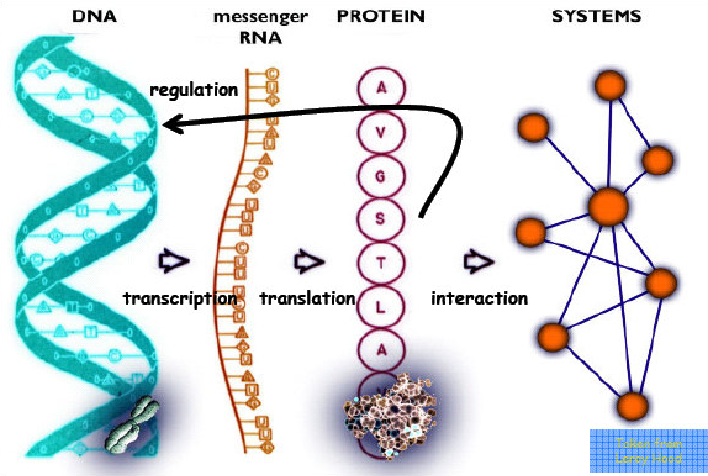
\includegraphics[height=3.5cm]{figs/dnascheme_white.png}
\end{center}

\pause
\begin{enumerate}[1)]
  \item Asynchronous Discrete Networks (ADN)
  \begin{itemize}
    \item[] Convenient to model biological systems
  \end{itemize}

  \smallskip
  \item Process Hitting (PH)
  \begin{itemize}
    \item[] Cannot accurately describe ADNs
  \end{itemize}

  \smallskip
  \item Enhancing PH with priorities
  \begin{itemize}
    \item[] To efficiently compute reachability in ADNs
  \end{itemize}
\end{enumerate}

\end{frame}


\section{Frameworks Definitions}
\subsection{Asynchronous Discrete Networks (ADN)}
% Définition du Réseaux Discrets Asynchrones

\newcommand{\Fadn}{\mathbb{F}}
\newcommand{\Eadn}{\mathbb{E}}
\newcommand{\SGadn}{\mathrm{G}}

\begin{frame}[c]
  \frametitle{The Asynchronous Discrete Networks (ADN)}
  \framesubtitle{\tcite{\citedejong}}

\begin{itemize}
  \item A set of components \qex{$N = \{ a, b, z \}$}
  \item A set of expression levels for each component \qex{$z \in \Fadn^z = \segm{0}{2}$}
  \item The set of global states \qex{$\Fadn = \Fadn^a \times \Fadn^b \times \Fadn^z$}
  \item An evolution function for each component \qex{$f^z : \Fadn \rightarrow \Fadn^z$}
\end{itemize}

\begin{center}
\begin{tabular}{ccc}
  \ex{$f^a = \neg b$} & \ex{$f^b = b \vee \neg a$} & \ex{$f^z = a + b$} \vspace{.5em}\\
  \begin{tabular}[t]{c|c}
    $b$ & $f^a(b)$ \\
  \hline
    $0$ & $\mathbf{1}$ \\
    $1$ & $\mathbf{0}$ \\
  \end{tabular}
&
  \begin{tabular}[t]{cc|c}
    $a$ & $b$ & $f^b(a, b)$ \\
  \hline
    $0$ & $0$ & $\mathbf{1}$ \\
    $0$ & $1$ & $\mathbf{1}$ \\
    $1$ & $0$ & $\mathbf{0}$ \\
    $1$ & $1$ & $\mathbf{1}$
  \end{tabular}
&
  \begin{tabular}[t]{cc|c}
    $a$ & $b$ & $f^z(a, b)$ \\
  \hline
    $0$ & $0$ & $\mathbf{0}$ \\
    $0$ & $1$ & $\mathbf{1}$ \\
    $1$ & $0$ & $\mathbf{1}$ \\
    $1$ & $1$ & $\mathbf{2}$
  \end{tabular}
\end{tabular}

\bigskip

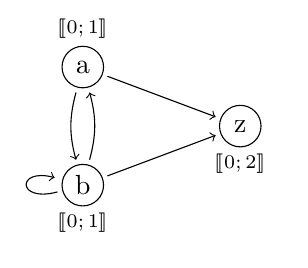
\begin{tikzpicture}[adn]
  \path[use as bounding box] (-0.7,-0.7) rectangle (2.5,2);
  \node[inner sep=0] (z) at (2,0.75) {z};
  \node[inner sep=0] (a) at (0,1.5) {a};
  \node[inner sep=0] (b) at (0,0) {b};
  \path
    node[elabel, above=-1em of a] {$\segm{0}{1}$}
    node[elabel, below=-1em of b] {$\segm{0}{1}$}
    node[elabel, below=-1em of z] {$\segm{0}{2}$};
  \path
    (a) edge[bend right=15] (b)
    (b) edge[bend right=15] (a)
    (b) edge[loop left] (b)
    (a) edge (z)
    (b) edge (z);
\end{tikzpicture}
\end{center}
\end{frame}



\begin{frame}[c]
  \frametitle{The Asynchronous Discrete Networks (ADN)}

State Graph: $\SGadn = (\Fadn, \Eadn)$, where one component evolves at a time given its function $f^a$
$$(x, y) \in \Eadn \Longleftrightarrow \exists a \in N, y^a = f^a(x) \wedge \forall b \neq a, y^b = x^b$$

%\f Only one component at a time $a$ evolves to reach the value of its evolution function $f^a(x)$

\pause
\medskip
%\begin{tabular*}{\textwidth}{@{\extracolsep{\fill}}lcc}
%  Size of the State Graph: & $\displaystyle|\Fadn| = \prod_{a \in N} |\Fadn^a| \quad\geq 2^{|N|}$ &
%\end{tabular*}
Size of the State Graph: \quad $\displaystyle|\Fadn| = \prod_{a \in N} |\Fadn^a| \quad\geq 2^{|N|}$

\medskip
\f Exponential in the number $|N|$ of components

\pause
\bigskip
Some works give a link between the structure and the behaviour of an ADN
\begin{itemize}
  \item \tval{Thomas' conjecture} (condition for multiple fixed points or attractive cycle)
  \begin{itemize}
    \item Boolean: \tcite{\citeremy}
    \item Multivalued: \tcite{\citerichardcomet}
  \end{itemize}
\end{itemize}

\pause
\medskip
But methods related to reachability rely on the State Graph

e.g.: \ex{Starting from $(a, b, z) = (0, 0, 0)$, can the system reach $z = 2$ ?}
\begin{itemize}
  \item \tval{Temporal logics}
  \begin{itemize}
    \item CTL: \tcite{\citesmbionet}
    \item LTL: \tcite{\citeito}
  \end{itemize}
\end{itemize}
\end{frame}

\subsection{The Process Hitting framework (PH)}
% Définition du Process Hitting + sortes coopératives

\begin{frame}[t]
  \frametitle{The Process Hitting modeling}
  \framesubtitle{\tcite{\citepmrtcsb}}

% 1 : Sortes
\only<1>{
\tikzstyle{process}=[circle,minimum size=15pt,font=\footnotesize,inner sep=1pt]
\tikzstyle{tick label}=[color=white, font=\footnotesize]
\tikzstyle{tick}=[transparent]
\tikzstyle{hit}=[transparent]
\tikzstyle{selfhit}=[transparent, min distance=30pt,curve to]
\tikzstyle{bounce}=[transparent]
\tikzstyle{hlhit}=[transparent]
\begin{center}\scalebox{\scaleex}{
\begin{tikzpicture}
  \exphdef
\end{tikzpicture}
}\end{center}
}

% 2 : Processus
\only<2>{
\tikzstyle{process}=[circle,draw,minimum size=15pt,font=\footnotesize,inner sep=1pt]
\tikzstyle{tick label}=[font=\footnotesize]
\tikzstyle{tick}=[densely dotted]
\tikzstyle{hit}=[transparent]
\tikzstyle{selfhit}=[transparent, min distance=30pt,curve to]
\tikzstyle{bounce}=[transparent]
\tikzstyle{hlhit}=[transparent]
\begin{center}\scalebox{\scaleex}{
\begin{tikzpicture}
  \exphdef
\end{tikzpicture}
}\end{center}
}

% 3 : États
\only<3>{
\tikzstyle{hit}=[transparent]
\tikzstyle{selfhit}=[transparent, min distance=30pt,curve to]
\tikzstyle{bounce}=[transparent]
\tikzstyle{hlhit}=[transparent]
\begin{center}\scalebox{\scaleex}{
\begin{tikzpicture}
  \exphdef

  \TState{3}{a_0,b_1,z_0}
\end{tikzpicture}
}\end{center}
}

% 4 : Actions
\only<4->{
\tikzstyle{tick}=[densely dotted]
\tikzstyle{hit}=[->,>=angle 45]
\tikzstyle{selfhit}=[min distance=30pt,curve to]
\tikzstyle{bounce}=[densely dotted,>=stealth',->]
\tikzstyle{hlhit}=[very thick]
\begin{center}\scalebox{\scaleex}{
\begin{tikzpicture}
  \exphdef

  \TState{4-5}{a_0,b_1,z_0}
  \TState{6}{a_0,b_1,z_1}
  \TState{7}{a_1,b_1,z_1}
  \TState{8}{a_1,b_1,z_2}

  \only<5>{
    \THit{b_1}{hl}{z_0}{.west}{z_1}
    \path[bounce,bend left,hl] \TBounce{z_0}{}{z_1}{.south};
  }
  \only<6>{
    \THit{a_0}{out=250,in=200,selfhit,hl}{a_0}{.west}{a_1}
    \path[bounce,bend left,hl] \TBounce{a_0}{}{a_1}{.south};
  }
  \only<7>{
    \THit{a_1}{hl}{z_1}{.west}{z_2}
    \path[bounce,bend left,hl] \TBounce{z_1}{}{z_2}{.south};
  }
\end{tikzpicture}
}\end{center}
}

\medskip
\begin{liste}
  \item \tval{Sorts}: components \qex{$a$, $b$, $z$}
\pause[2]
  \item \tval{Processes}: local states / levels of expression \qex{$z_0$, $z_1$, $z_2$}
\pause[3]
  \item \tval{States}: sets of active processes%
  \only<3-5>{\qex{$\PHetat{a_0, b_1, z_0}$}}%
  \only<6>{\qex{$\PHetat{a_0, b_1, z_1}$}}%
  \only<7>{\qex{$\PHetat{a_1, b_1, z_1}$}}%
  \only<8>{\qex{$\PHetat{a_1, b_1, z_2}$}}%
\pause[4]
  \item \tval{Actions}: dynamics \qex{\only<5>{\underline}{$\PHfrappe{b_1}{z_0}{z_1}$}, \only<6>{\underline}{$\PHfrappe{a_0}{a_0}{a_1}$}, \only<7>{\underline}{$\PHfrappe{a_1}{z_1}{z_2}$}}
\end{liste}
\end{frame}

% Analyse statique

\subsubsection{Successive reachability}

\begin{frame}[t]
  \frametitle{Static analysis: successive reachability of processes}
  \framesubtitle{\tcite{\citepmrmscs}}

%Successive reachability of processes:

\begin{columns}
\begin{column}{0.55\textwidth}

\begin{center}
\scalebox{0.75}{
\begin{tikzpicture}
  %\path[use as bounding box] (-1,-3) rectangle (7,2);
  \exatt

  \TState{2-4}{a_0,b_0,b_2,c_0,d_0}

  \TState{5}{a_0,b_0,c_0,d_0}
  \TState{6}{a_0,b_0,c_1,d_0}
  \TState{7}{a_0,b_0,c_1,d_1}
  \TState{8}{a_0,b_1,c_1,d_1}
  \TState{9}{a_0,b_1,c_1,d_2}

  \node<3>[process,very thick] (d_1) at (d_1.center) {1?};
  \node<3>[process,very thick] (b_1) at (b_1.center) {2?};
  \node<3>[process,very thick] (d_2) at (d_2.center) {3?};

  \node<4-8>[process,very thick,fill=none] (d_2) at (d_2.center) {1?};
  \node<9>[process,very thick,fill=none] (d_2) at (d_2.center) {};

  \only<5>{\THit{a_0}{hlhit}{c_0}{.north}{c_1}}
  \path<5>[bounce,bend left,hlhit] \TBounce{c_0}{}{c_1}{.west};
  \only<6>{\THit{b_0}{hlhit}{d_0}{.west}{d_1}}
  \path<6>[bounce,bend left,hlhit] \TBounce{d_0}{}{d_1}{.south};
  \only<7>{\THit{c_1}{bend left=20pt,hlhit}{b_0}{.west}{b_1}}
  \path<7>[bounce,bend left,hlhit] \TBounce{b_0}{}{b_1}{.south};
  \only<8>{\THit{b_1}{hlhit}{d_1}{.west}{d_2}}
  \path<8>[bounce,bend left,hlhit] \TBounce{d_1}{}{d_2}{.south};
\end{tikzpicture}
}
\end{center}

\end{column}
\begin{column}{0.45\textwidth}

\pause
~\\~\\~\\~\\
\begin{itemize}
  \item Initial context
    \\ \rex{\PHetat{a_1, \{b_0, b_1\}, c_0, d_0}} \pause
  \item Objectives
    \\ \rex{$[\ \Rsh d_1 \PHconcat\ \Rsh b_1 \PHconcat\ \Rsh d_2\ ]$} \pause
    \\\smallskip \rex{$[\ \Rsh d_2\ ]$} \pause
\end{itemize}

\end{column}
\end{columns}

\medskip
\begin{center}
\f Concretization of the objective = scenario

\ex{
$ \only<5>{\underline{\PHfrappe{a_0}{c_0}{c_1}}} \only<-4,6->{\PHfrappe{a_0}{c_0}{c_1}} \PHconcat %
  \only<6>{\underline{\PHfrappe{b_0}{d_0}{d_1}}}\only<-5,7->{\PHfrappe{b_0}{d_0}{d_1}} \PHconcat %
  \only<7>{\underline{\PHfrappe{c_1}{b_0}{b_1}}}\only<-6,8->{\PHfrappe{c_1}{b_0}{b_1}} \PHconcat %
  \only<8>{\underline{\PHfrappe{b_1}{d_1}{d_2}}}\only<-7,9->{\PHfrappe{b_1}{d_1}{d_2}}
$}
\end{center}
\end{frame}



\begin{frame}
  \frametitle{Over- and Under-approximations}
  \framesubtitle{\tcite{\citepmrmscs}}

Static analysis by abstractions:
\begin{fleches}
  \item Directly checking an objective sequence $R$ is hard (\tval{State Graph})
  \item Rather check the approximations $P$ and $Q$, where $P \Rightarrow R \Rightarrow Q$:
\end{fleches}

\begin{center}
\scalebox{0.7}{
  \figsa
}
\end{center}

\uncover<8->{
%Polynomial w.r.t.~the number of sorts and \\exponential w.r.t.~the number of processes in each sort
Computing $P$ or $Q$ is \tval{polynomial} in the number of \tval{sorts} \\and \tval{exponential} in the number of \tval{processes in each sort}
\begin{fleches}
  \item Efficient for big models with few levels of expression
\end{fleches}
}
\end{frame}

% Exemples de structures abstraites (graphes de causalité locale)

\begin{frame}
  \frametitle{Under-approximation}

\def \tu {2}
\def \tub {3}
\def \tuf {4}

\begin{columns}
\begin{column}{0.48\textwidth}
\begin{center}
\scalebox{0.55}{
\begin{tikzpicture}
\exatt
\TState{-\tu}{a_1,b_1,c_1,d_0}
\TState{\tub-}{a_0,b_1,c_0,d_0}
\node[process,very thick] (d_2) at (d_2.center) {?};
\end{tikzpicture}
}
\end{center}

\end{column}
\begin{column}{0.52\textwidth}

\vspace{1.5em}
\tval{Sufficient condition}:

\smallskip
\begin{itemize}
  \item no cycle
  \item \only<-\tu>{each objective has a solution} \only<\tub->{\sout{each objective has a solution}}
\end{itemize}
\begin{center}
  \only<\tu>{\Large\textcolor{darkgreen}{$R$ is \textbf{true}}} \only<\tuf>{\Large\textcolor{darkyellow}{\textbf{Inconclusive}}}
\end{center}

\end{column}
\end{columns}

\only<-\tu>{
\sauyes
}

\only<\tub->{
\sauinconc
}

\end{frame}



\begin{frame}
  \frametitle{Over-approximation}

\def \to {4}
\def \tob {5}
\def \tof {6}
\def \tokp {7}

\begin{columns}
\begin{column}{0.48\textwidth}
\begin{center}
\scalebox{0.55}{
\begin{tikzpicture}
\exatt
\TState{-\to}{a_1,b_0,c_0,d_1}
\TState{\tob-}{a_1,b_1,c_1,d_0}
\node[process,very thick] (d_2) at (d_2.center) {?};
\end{tikzpicture}
}
\end{center}
\bigskip

\end{column}
\begin{column}{0.52\textwidth}

\tval{Necessary condition}:

\smallskip
\only<2->{
\only<3-\to>{\sout{There exists a traversal}}\only<2,\tob->{There exists a traversal}
with no cycle

\smallskip
\begin{itemize}
  \item \only<3-\to>{\sout{objective $\rightarrow$ follow one solution}}\only<1-2,\tob->{objective $\rightarrow$ follow one solution}
  \item solution $\rightarrow$ follow all processes
  \item process $\rightarrow$ follow all objectives
\end{itemize}
\begin{center}
  \only<\to>{\Large\textcolor{red}{$R$ is \textbf{false}}}\only<\tof->{\Large\textcolor{darkyellow}{\textbf{Inconclusive}}}
\end{center}
}

\end{column}
\end{columns}

%\bigskip

\only<1-\to>{
\saono
}

\only<\tob->{
\saoinconc
}

\end{frame}

% Conclusion sur le Process Hitting

\begin{comment}
  \frametitle{The Process Hitting modeling}

\todo{À réorganiser}

\begin{itemize}
  \item \tval{Dynamic} modeling with an \tval{atomistic} point of view
  \begin{fleches}
    \item Independent actions
    \item Cooperation modeled with cooperative sorts
  \end{fleches}

  \smallskip
  \item Efficient \tval{static analysis}
  \begin{fleches}
    \item Reachability of a process can be computed in \tval{polynomial time}\\
          \quad in the number of sorts
  \end{fleches}

  \smallskip
  \item Useful for the study of \tval{large biological models}
  \begin{fleches}
    \item Up to hundreds of sorts
    \item With few expression levels (Boolean or multivalued with $n \leq 4$)
  \end{fleches}

  \smallskip
  \item (Future) extensions
  \begin{fleches}
    \item Actions with priorities
    \item Continuous time with clocks?
  \end{fleches}
\end{itemize}

\end{comment}



\begin{frame}[c]
  \frametitle{Implementation in \Pint{}}

\begin{center}
  \tval{Existing free OCaml library:} \Pint
\end{center}

\medskip
\f Compiler + tools for Process Hitting models

\f Documentation \& examples: \lien{http://processhitting.wordpress.com/}

\pause
\bigskip
\medskip
\tval{Computation time for various reachability analyses:}

\medskip
\small
\begin{tabular}{r||c|c|c|c||c|c|c|}
\hline
\tval{Model} & Sorts & Procs & Actions & States & Biocham$^1$ & libddd$^2$ & \Pint \\\hline
\tval{\ex{egfr20}} & 35 & 196 & 670 & $2^{64}$ & [3s -- $\infty$] & [1s -- 150s] & \tval{0.007s} \\\hline
\tval{\ex{tcrsig40}} & 54 & 156 & 301 & $2^{73}$ & [1s -- $\infty$] & [0.6s -- $\infty$] & \tval{0.004s} \\\hline
\tval{\ex{tcrsig94}} & 133 & 448 & 1124 & $2^{194}$ & $\infty$ & $\infty$ & \tval{0.030s} \\\hline
\tval{\ex{egfr104}} & 193 & 748 &  2356 & $2^{320}$ &  $\infty$ & $\infty$ & \tval{0.050s}\\\hline
\end{tabular}

\medskip
\quad$^1$ Inria Paris-Rocquencourt/Contraintes\\
\quad$^2$ LIP6/Move

\citemodels

\end{frame}


\section{Adding priorities to the Process Hitting}
% Ajout des actions prioritaires pour avoir une équivalence avec les ADN

\begin{frame}
  \frametitle{Adding cooperations}
  \framesubtitle{\tcite{\citepmrtcsb}}

\begin{center}\scalebox{\scaleex}{
\begin{tikzpicture}
  \exphcoop
  
  \TState{9}{a_1,b_1}
  \TState{10}{a_1,b_1,ab_0}
  \TState{11}{a_1,b_1,ab_1}
  \TState{12}{a_1,b_1,ab_3}
  
  \only<9>{
    \node[hl process] at (ab_0.center) {};
    \node[hl process] at (ab_1.center) {};
    \node[hl process] at (ab_2.center) {};
    \node[current process] at (ab_3.center) {};
  }
  
  \only<10>{
    \THit{b_1}{hl}{ab_0}{.210}{ab_1}
    \path[bounce,bend left,hl] \TBounce{ab_0}{}{ab_1}{.240} ;
  }
  
  \only<11>{
    \THit{a_1}{hl}{ab_1}{.160}{ab_3}
    \path[bounce,bend left,hl] \TBounce{ab_1}{}{ab_3}{.south west} ;
  }
\end{tikzpicture}
}\end{center}

\medskip
%\only<-14>{
\begin{liste}
  \item \tval{Cooperation} between \ex{$a_1$} and \ex{$b_1$}: \qex{$\PHfrappe{[a_1 \wedge b_1]}{z_0}{z_1}$}
\pause[5]
  \item Solution: a \tval{cooperative sort} \qex{$ab$} \only<12->{\quad to express \qex{$a_1 \wedge b_1$}}
\pause[9]
  \item Constraint: each configuration is represented by one process \qex{$\PHetat{a_1,b_1} \Rightarrow ab_{11}$}
%\pause[15]
%  \item Advantage: regular sort; drawbacks: complexity, temporal shift
\end{liste}%}
\end{frame}



\begin{frame}
  \frametitle{Adapting the expressivity of PH}
  \framesubtitle{~}

\begin{center}\scalebox{\scaleex}{
\begin{tikzpicture}
  \path[use as bounding box] (-0.5,-0.5) rectangle (6.5,4.5);
  %\path[use as bounding box] (-1,-0.5) rectangle (7.5,5);

  \exphcoopprio{unprio}{}

  \only<2>{
    \THit{a_1}{selfhit,hlb}{a_1}{.west}{a_0}
    \path[bounce,bend right,hlb] \TBounce{a_1}{}{a_0}{.north west} ;
  }
  \only<3>{
    \THit{b_0.south west}{bend left=90,hlb}{a_0}{.west}{a_1}
    \path[bounce,bend left,hlb] \TBounce{a_0}{}{a_1}{.south west} ;
  }
  \only<4>{
    \THit{b_1}{selfhit,hlb}{b_1}{.west}{b_0}
    \THit{a_0}{bend right=50,hlb}{b_0}{.west}{b_1}
    \path[bounce,bend right,hlb] \TBounce{b_1}{}{b_0}{.north west} ;
    \path[bounce,bend left,hlb] \TBounce{b_0}{}{b_1}{.south west} ;
  }

  \TState{5}{a_0, b_0, ab_0, z_0}
  \only<5>{
  \THit{b_0.south west}{hl,bend left=90}{a_0}{.west}{a_1}
  \path[bounce,bend left,hl] \TBounce{a_0}{}{a_1}{.south west} ;
  }
  \TState{6}{a_1, b_0, ab_0, z_0}
  \only<6>{
  \THit{a_1}{hl}{ab_0}{.west}{ab_2}
  \path[bounce,bend left,hl] \TBounce{ab_0}{}{ab_2}{.240} ;
  }
  \TState{7}{a_1, b_0, ab_2, z_0}
  \only<7>{
  \THit{a_1}{selfhit,hl}{a_1}{.west}{a_0}
  \path[bounce,bend right,hl] \TBounce{a_1}{}{a_0}{.north west} ;
  }
  \TState{8}{a_0, b_0, ab_2, z_0}
  \only<8>{
  \THit{a_0}{bend right=50,hl}{b_0}{.west}{b_1}
  \path[bounce,bend left,hl] \TBounce{b_0}{}{b_1}{.south west} ;
  }
  \TState{9}{a_0, b_1, ab_2, z_0}
  \only<9>{
  \THit{b_1}{hl}{ab_2}{.200}{ab_3}
  \path[bounce,bend left,hl] \TBounce{ab_2}{}{ab_3}{.south} ;
  }
  \TState{10}{a_0, b_1, ab_3, z_0}
  \only<10>{
  \THit{ab_3}{hl}{z_0}{.west}{z_1}
  \path[bounce,bend left,hl] \TBounce{z_0}{}{z_1}{.south} ;
  }
  \TState{11-}{a_0, b_1, ab_3, z_1}
\end{tikzpicture}
}\end{center}

\medskip

\tval{Drawback}: Cooperations are too “loose” to be as expressive as ADN.

\medskip

$ \uncover<5->{\PHstate{a_0, b_0, ab_{00}, z_0}}
  \uncover<6->{\rightarrow\PHstate{a_1, b_0, ab_{00}, z_0}}
  \uncover<7->{\rightarrow\PHstate{a_1, b_0, ab_{10}, z_0}}
  \uncover<8->{\rightarrow\PHstate{a_0, b_0, ab_{10}, z_0}}$
\\ \qquad
$ \uncover<9->{\rightarrow\PHstate{a_0, b_1, ab_{10}, z_0}}
  \uncover<10->{\rightarrow\PHstate{a_0, b_1, \redex{ab_{11}}, z_0}}
  \uncover<11->{\rightarrow\PHstate{a_0, b_1, \redex{ab_{11}}, \redex{z_1}}}$

\medskip

\uncover<12->{
The cooperativity should be: \qex{$a_1 \wedge b_1$ simultaneously}

but the model behaves like: \qex{$\mathbf{P}(a_1) \wedge \mathbf{P}(b_1)$} \quad with $\mathbf{P}$ = “previously”
}

\end{frame}



\begin{frame}
  \frametitle{Adapting the expressivity of PH}
  \framesubtitle{~}

\begin{center}\scalebox{\scaleex}{
\begin{tikzpicture}
  \path[use as bounding box] (-0.5,-0.5) rectangle (6.5,4.5);

  \exphcoopprio{prio}{}

  \TState{3}{a_0, b_0, ab_0, z_0}
  \only<3>{
  \THit{b_0.south west}{hl,bend left=90}{a_0}{.west}{a_1}
  \path[bounce,bend left,hl] \TBounce{a_0}{}{a_1}{.south west} ;
  }
  \TState{4}{a_1, b_0, ab_0, z_0}
  \only<4>{
  \THit{a_1}{prio,hl}{ab_0}{.west}{ab_2}
  \path[bounce,bend left,hl] \TBounce{ab_0}{}{ab_2}{.240} ;
  }
  \TState{5}{a_1, b_0, ab_2, z_0}
  \only<5>{
  \THit{a_1}{selfhit,hl}{a_1}{.west}{a_0}
  \path[bounce,bend right,hl] \TBounce{a_1}{}{a_0}{.north west} ;
  }
  \TState{6}{a_0, b_0, ab_2, z_0}
  \only<6>{
  \THit{a_0}{prio,hl}{ab_2}{.160}{ab_0}
  \path[bounce,bend right,hl] \TBounce{ab_2}{}{ab_0}{.north west} ;
  }
  \TState{7}{a_0, b_0, ab_0, z_0}
  \only<7>{
  \THit{a_0}{bend right=50,hl}{b_0}{.west}{b_1}
  \path[bounce,bend left,hl] \TBounce{b_0}{}{b_1}{.south west} ;
  }
  \TState{8}{a_0, b_1, ab_0, z_0}
  \only<8>{
  \THit{b_1}{prio,hl}{ab_0}{.210}{ab_1}
  \path[bounce,bend left] \TBounce{ab_0}{hl}{ab_1}{.240} ;
  }
  \TState{9-}{a_0, b_1, ab_1, z_0}
\end{tikzpicture}
}\end{center}

\begin{itemize}
  \item Prioritise actions updating cooperative sorts (non-biological actions)
  \item All other actions remain unprioritised (evolutions with delays)
\end{itemize}
\pause
\F Whenever a regular action is played, all cooperative sorts are already updated

%\medskip
%Now, $z_1$ cannot be reached from $\PHstate{a_0, b_0, ab_{00}, z_0}$

\medskip
$ \uncover<3->{\PHstate{a_0, b_0, ab_{00}, z_0}}
  \uncover<4->{\rightarrow\PHstate{a_1, b_0, ab_{00}, z_0}}
  \uncover<5->{\rightarrow\PHstate{a_1, b_0, ab_{10}, z_0}}
  \uncover<6->{\rightarrow\PHstate{a_0, b_0, ab_{10}, z_0}}$
\\ \qquad
$ \uncover<7->{\rightarrow\PHstate{a_0, b_0, \ex{ab_{00}}, z_0}}
  \uncover<8->{\rightarrow\PHstate{a_0, b_1, \ex{ab_{00}}, z_0}}
  \uncover<9->{\rightarrow\PHstate{a_0, b_1, \ex{ab_{01}}, z_0}}$

\end{frame}


% Analyse statique avec priorités

\begin{frame}[c]
  \frametitle{Static analysis with prioritised actions}

\tval{Sufficient condition:}

\begin{itemize}
  \item no cycle
  \item each objective has a solution
  \item \only<-4>{coherent edges}\only<5->{\sout{coherent edges}}
\end{itemize}
\vspace{1cm}
\hspace{2cm}\uncover<5->{\textcolor{darkyellow}{\textbf{Inconclusive}}}
\vspace{-3cm}

\begin{center}\scalebox{\scaleex}{
\begin{tikzpicture}[aS]
  \priostatic

  \path<2-5> (ab11) edge[aSPrio,Aex] (ab11s);
  \path<5-> (ab11) edge[aSPrio,Ahledge] (ab11s);

  \node<3>[Aproc,Aex,at=(a1)] {$a_1$};
  \node<3>[Aproc,Aex,at=(b1)] {$b_1$};
  \node<4->[Aproc,Ahl,at=(a1)] {$a_1$};
  \node<4->[Aproc,Ahl,at=(a0)] {$a_0$};
  %\node<2>[Aproc,Ahl,at=(b0)] {$b_0$};
  %\node<2>[Aproc,Ahl,at=(b1)] {$b_1$};
\end{tikzpicture}
}\end{center}

\scalebox{\scaleminiex}{
\begin{tikzpicture}
  \path[use as bounding box] (-0.5,-0.5) rectangle (8.5,3.5);
  \tikzstyle{current process}=[process,fill=gray]
  \exphcoopprio{prio}{}
  \node[process,very thick] at (z_1.center) {?};
  \TState{1-}{a_0, b_0, ab_0, z_0}
\end{tikzpicture}}
\hfill
\scalebox{\scaleex}{
\scalebox{\scaleex}{
\begin{tikzpicture}[aS]
  \path[use as bounding box] (0,0) rectangle (5.8,4);
  \glclegend{prio}{$z_1$}{$\PHobj{z_0}{z_1}$}
\end{tikzpicture}
}}

\end{frame}



\section{Summary \& Conclusion}
% Performances et conclusion

\begin{frame}[c]
  \frametitle{Implementation}

Complexity:

\begin{itemize}
  \item Building the graph:
  \begin{itemize}
    \item Polynomial in the number of sorts
    \item Exponential in the number of processes in each sort
  \end{itemize}
  \item Analysing the graph:
  \begin{itemize}
    \item Polynomial in the size of the graph
  \end{itemize}
\end{itemize}

\pause
\bigskip
\small
\begin{tabular}{r||c|c|c|c||c|c|c|}
\hline
\tval{Model} & Sorts & Procs & Actions & States & libddd$^1$ & GINsim$^2$ & \Pint \\\hline
\tval{\ex{egfr20}} & 35 & 196 & 670 & $2^{64}$ & & $<$1s & \tval{0.35s} \\\hline
\tval{\ex{tcrsig40}} & 54 & 156 & 301 & $2^{73}$ & & $\infty$ & \tval{0.2s} \\\hline
\tval{\ex{tcrsig94}} & 133 & 448 & 1124 & $2^{194}$ & [13min -- $\infty$] & & \tval{0.8s} \\\hline
%\tval{\ex{egfr104}} & 193 & 748 &  2356 & $2^{320}$ &  $\infty$ & $\infty$ & \tval{0.050s}\\\hline
\end{tabular}

\medskip
\quad$^1$ LIP6/Move\\
\quad$^2$ TAGC/IGC

%S = Sorts \quad CS = Cooperative sorts \quad P = Processes \quad A = Actions

%\cmodels
\bigskip
\citeegfra\\
\citetcrsiga\\
\citetcrsigb\\
\end{frame}



\begin{frame}[c]
  \frametitle{Summary}

\begin{itemize}
  \item The Process Hitting framework
  \begin{fleches}
    \item Restricted concurrent actions
    \item Efficient static analysis on biological models (few expression levels)
  \end{fleches}
  
  \smallskip
  \item But raw Process Hitting is insufficient to models ADNs
  \begin{fleches}
    \item How to represent cooperations?
    \item Cooperative sorts only represent a combination of past states
  \end{fleches}
  
  \smallskip
  \item Solution: prioritised actions
  \begin{fleches}
    \item Accurate cooperative sorts
    \item Expressivity of ADN is reached
  \end{fleches}
\end{itemize}
\end{frame}



\begin{frame}[c]
  \frametitle{Conclusion}

\begin{itemize}
  \item Achieved:
  \begin{itemize}
    \item Rise the expressivity of PH
    \item Efficient reachability analysis in ADNs
  \end{itemize}
  
  \smallskip
  \item Value:
  \begin{itemize}
    \item Model a whole class of ADNs in one PH model
    \item Efficiently analyse reachability for the whole class
    \item Refine the PH model to match desired behaviour
    \item Infer the underlying class of ADNs\\\quad\tcite{\citefpimrcmsb}
  \end{itemize}
\end{itemize}



\pause
\bigskip
\begin{flushright}
\Large
\textcolor{couleurtheme}{Outlook}\hspace*{2.7em}
\end{flushright}

\begin{itemize}
  \item Allow prioritised actions even for biological evolutions
  \item Allow $n>2$ classes of priority
  %\item $2$ priorities: first attempt to add priorities in the PH framework
\end{itemize}
\qquad~\f Model actions with delays by using priorities
\end{frame}


\appendix
\section[x]{Bibliography}
% Bibliographie

\begin{frame}[c]
  \frametitle{Bibliography}

\footnotesize
\setlength{\parindent}{-1em}
\setlength{\parskip}{0.5em}
~

\vfill

\tcitebullet Loïc Paulevé, Morgan Magnin, Olivier Roux. \ex{Refining dynamics of gene regulatory networks in a stochastic $\pi$-calculus framework}. In Corrado Priami, Ralph-Johan Back, Ion Petre, and Erik de Vink, editors: \textit{Transactions on Computational Systems Biology XIII}, Lecture Notes in Computer Science, 171-191. Springer Berlin Heidelberg, 2011.

\tcitebullet Loïc Paulevé, Morgan Magnin, Olivier Roux. \ex{Static analysis of biological regulatory networks dynamics using abstract interpretation}. \textit{Mathematical Structures in Computer Science}. 2012.

%\tcite{RCB08} Adrien Richard, Jean-Paul Comet, Gilles Bernot. \ex{R. Thomas' logical method}, 2008. Invited at \textit{Tutorials on modelling methods and tools: Modelling a genetic switch and Metabolic Networks}, Spring School on Modelling Complex Biological Systems in the Context of Genomics.

%\tcite{RCB06} Adrien Richard, Jean-Paul Comet, Gilles Bernot. \textit{Modern Formal Methods and App.}, chapter \ex{Formal Methods for Modeling Biological Regulatory Networks}, 83--122. 2006.

\tcitebullet Hidde de Jong. \ex{Modeling and simulation of genetic regulatory systems: a literature review}, \textit{Journal of Computational biology} 9(1), 67--103. 2002.

\tcitebullet Adrien Richard and Jean-Paul Comet. \ex{Necessary conditions for multistationarity in discrete dynamical systems}. \textit{Discrete Applied Mathematics} 155(18), 2403--2413. 2007.

\tcitebullet Élisabeth Remy, Paul Ruet and Denis Thieffry. \ex{Graphic requirements for multistability and attractive cycles in a boolean dynamical framework}, \textit{Advances in Applied Mathematics} 41(3), 335-350. Elsevier, 2008.

\tcitebullet Gilles Bernot, Jean-Paul Comet, Adrien Richard and Janine Guespin. \ex{Application of formal methods to biological regulatory networks: extending Thomas' asynchronous logical approach with temporal logic}, \textit{Journal of Theoretical Biology}, 229(3), 339--347. Elsevier, 2004.

\tcitebullet Sohei Ito, Naoko Izumi, Shigeki Hagihara and Naoki Yonezaki. \ex{Qualitative analysis of gene regulatory networks by satisfiability checking of Linear Temporal Logic}, in 2010 IEEE International Conference on \textit{BioInformatics and BioEngineering} (BIBE), 232--237. IEEE, 2010.

\tcitebullet Maxime Folschette, Loïc Paulevé, Katsumi Inoue, Morgan Magnin, Olivier Roux. \ex{Concretizing the Process Hitting into Biological Regulatory Networks}. In David Gilbert and Monika Heiner, editors, \textit{Computational Methods in Systems Biology X}, Lecture Notes in Computer Science, 166--186. Springer Berlin Heidelberg, 2012.

%\tcite{Paulevé11} Loïc Paulevé. PhD thesis: \ex{\textit{Modélisation, Simulation et Vérification des Grands Réseaux de Régulation Biologique}}, October 2011, Nantes, France

%\tcite{PMR10-TSE} Loïc Paulevé, Morgan Magnin, and Olivier Roux. \textit{Tuning Temporal Features within the Stochastic $\pi$-Calculus}. IEEE Transactions on Software Engineering, 37(6):858-871, 2011.

%\tcite{PR10-CRAS} Loïc Paulevé and Adrien Richard. \textit{Topological Fixed Points in Boolean Networks}. Comptes Rendus de l'Académie des Sciences - Series I - Mathematics, 348(15-16):825 - 828, 2010.

\vfill
\Large
\begin{flushright}
  \tval{Thank you}\hspace{1cm}~
\end{flushright}
\vfill

~

\end{frame}

%\section[Annex: Graphs of local causality]{Graphs of local causality}
%\input{parts/annex_ph.tex}



\end{document}
